
\section{Teori}

    \textbf{Motivasjon og sammenheng:} For å forstå hvorfor det er en grense på 100 meter for Ethernet-kabler, og hvordan signaler dempes og forvrenges i slike kabler, må vi bruke telegraflikningen. Denne beskriver hvordan elektriske signaler forplanter seg i transmisjonslinjer, og gir oss verktøyene til å analysere tap, dispersjon og gruppeforsinkelse.

\subsection{Fourierrekker og Fouriertransformasjon}

Mange signaler kan brytes ned i sine frekvenskomponenter ved hjelp av Fourier-analyse. Dette er spesielt nyttig i signalbehandling og for å forstå hvordan ulike frekvenser påvirkes av transmisjonslinjen. Vi bruker Fourier-rekker for endelige intervaller (Dirichlet/Neumann) og FFT for målt/simulert tidsserie, slik at vi kan hente ut overføringsfunksjonen $H(\omega)$, innsettingstap $IL(f)$ og gruppeforsinkelse $\tau_g(f)$.\\[1em]
En periodisk funksjon $f(t)$ med periode $T$ kan uttrykkes som en Fourier-rekke:
\begin{equation}
f(t) = a_0 + \sum_{n=1}^{\infty} \left( a_n \cos\left(\frac{2\pi n t}{T}\right) + b_n \sin\left(\frac{2\pi n t}{T}\right) \right)
\end{equation}
med koeffisienter gitt ved:
\begin{align*}
a_0 &= \frac{1}{T} \int_{0}^{T} f(t) \, dt \\
a_n &= \frac{2}{T} \int_{0}^{T} f(t) \cos\left(\frac{2\pi n t}{T}\right) dt \\
b_n &= \frac{2}{T} \int_{0}^{T} f(t) \sin\left(\frac{2\pi n t}{T}\right) dt
\end{align*}
Fouriertransformasjonen gir oss signalets spektrum:
\begin{equation}
F(\omega) = \int_{-\infty}^{\infty} f(t) e^{-j\omega t} dt
\end{equation}
og den inverse transformasjonen:
\begin{equation}
f(t) = \frac{1}{2\pi} \int_{-\infty}^{\infty} F(\omega) e^{j\omega t} d\omega
\end{equation}
I praksis bruker vi diskret Fourier-transformasjon (DFT) og spesielt FFT for å analysere målt/simulert tidsserie og hente ut $H(f)$ og $\tau_g(f)$.

\clearpage
\subsection{Telegraflikningen og transmisjonslinjer}

Telegraflikningen gir en matematisk modell for hvordan spenning og strøm forplanter seg i en transmisjonslinje, som for eksempel en Ethernet-kabel. Den tar hensyn til både resistive og reaktive elementer, og forklarer hvorfor signaler dempes og forvrenges over avstand og tid.
Vi ser på et uendelig lite stykke av en transmisjonslinje som en elektrisk krets bestående av motstand $R dx$, induktans $L dx$, konduktans $G dx$ og kapasitans $C dx$, se Figur~\ref{fig:telegraflinje}.

\begin{figure}[h]
    \centering
    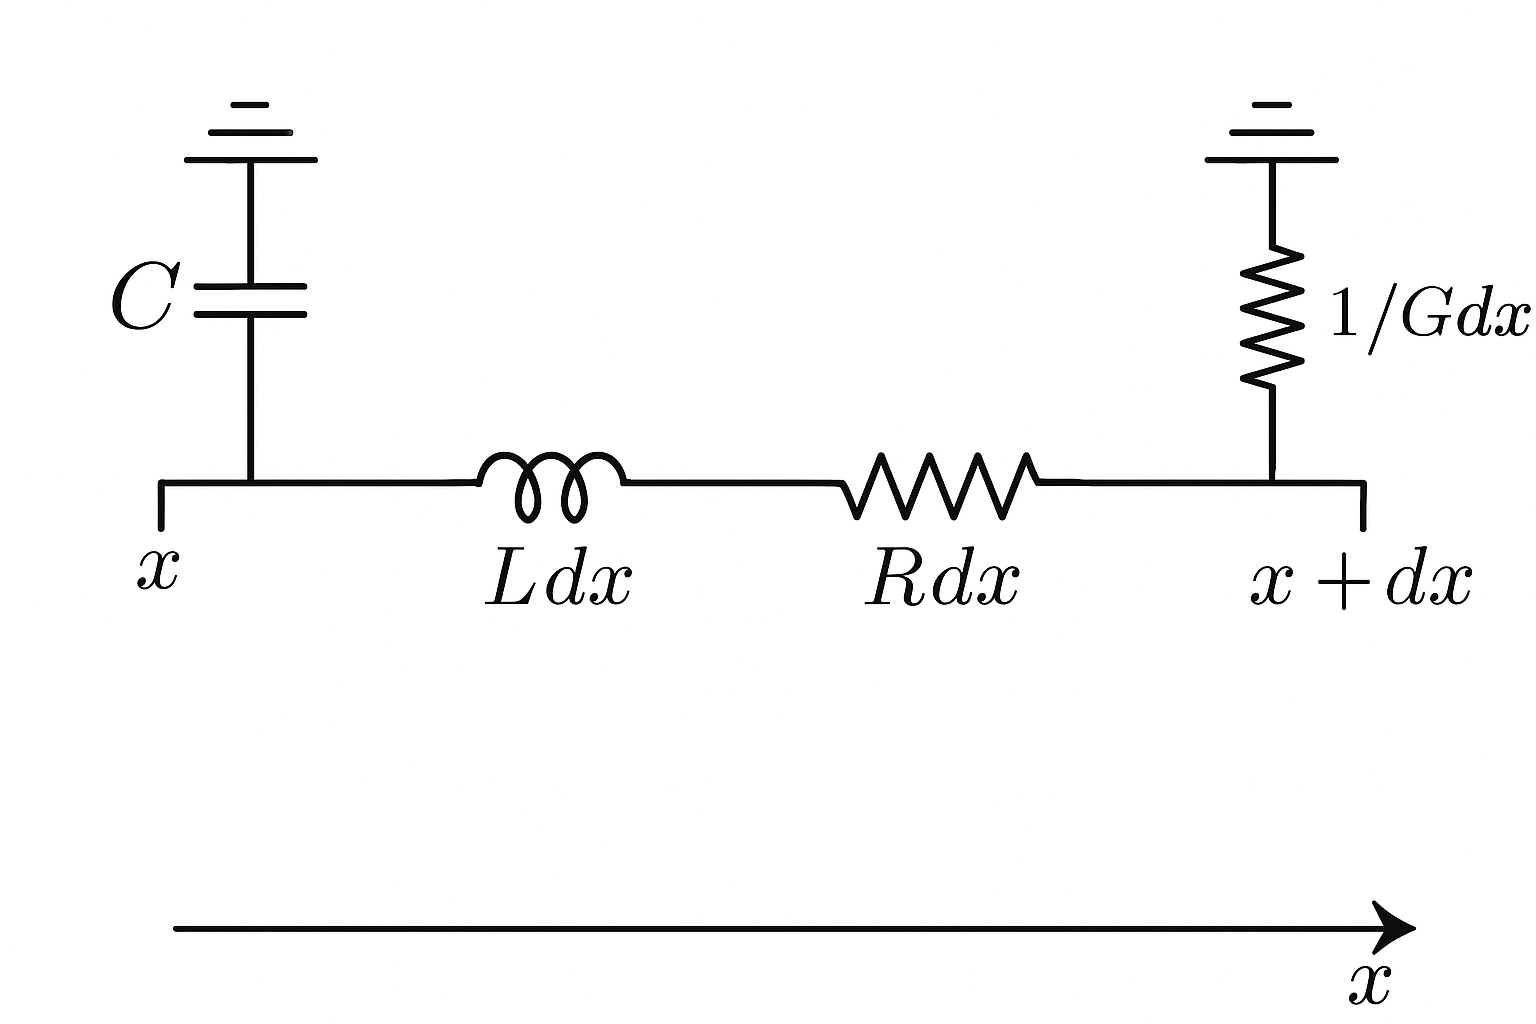
\includegraphics[width=0.7\textwidth]{Media/telegraflinje.png}
    \caption{Elementært stykke av transmisjonslinje med parametrene $R$, $L$, $G$, og $C$.}
    \label{fig:telegraflinje}
\end{figure}

\noindent Ved å bruke Kirchhoffs lover får vi differensiallikningene:
\begin{align}
u_x + R i + L i_t &= 0 \\
C u_t + G u + i_x &= 0
\end{align}
Disse kan kombineres til telegraflikningen:
\begin{equation}
u_{tt} + (\alpha + \beta) u_t + \alpha \beta u = c^2 u_{xx}
\end{equation}
hvor
\begin{align*}
c^2 &= \frac{1}{LC} \\
\alpha &= \frac{G}{C} \\
\beta &= \frac{R}{L}
\end{align*}
Her er $R$, $L$, $G$, $C$ motstand, induktans, konduktans og kapasitans per lengdeenhet. Denne likningen danner grunnlaget for å forstå tap, dispersjon og maksimal kabellengde i praksis.

\subsubsection{Metoder og praktisk relevans}

(a) \textit{Fourierrekker:} Analytisk på $[0,L]$ (m/Dirichlet) for å vise $\alpha=\beta$-tilfellet.\\
(b) \textit{FFT:} Fouriertransform numerisk for å hente $H(f)$ og $\tau_g(f)$ fra tidsserier.

\subsubsection{Dispersjon og gruppeforsinkelse}

Dispersjon betyr at ulike frekvenskomponenter i en bølge forplanter seg med forskjellig hastighet. Dette fører til at signaler forvrenges når de forplanter seg langt. Gruppeforsinkelsen er gitt ved:
\clearpage
\dots

\begin{equation}
	au_g(\omega) = \frac{d\beta}{d\omega} L \approx \frac{L}{v} \quad \text{(lavtaps)}
\end{equation}

\subsubsection{Oppsummering og kobling til prosjektet}

Teorien over forklarer hvorfor signaler i lange kabler dempes og forvrenges, og gir oss verktøyene til å analysere dette både analytisk og numerisk. Dette er avgjørende for å forstå hvorfor det er en 100 m-grense for Ethernet-kabler. I det videre arbeidet skal vi først gjennomføre praktiske målinger, og deretter numeriske simuleringer, slik at begge kan sammenlignes med de teoretiske resultatene for å se hvordan modellen stemmer med virkeligheten.